\documentclass[aspectratio=169]{beamer}

\usepackage{mystyle}

%Concepts
\newcommand{\iot}{IoT\xspace}
\newcommand{\iomt}{IoMT\xspace}
\newcommand{\software}{software\xspace}
\newcommand{\Software}{Software\xspace}
\newcommand{\middleware}{middleware\xspace}
\newcommand{\Middleware}{Middleware\xspace}
\newcommand{\smartobj}{\textit{smart object}\xspace}
\newcommand{\Smartobj}{\textit{Smart object}\xspace}
\newcommand{\smartobjs}{\textit{smart objects}\xspace}
\newcommand{\Smartobjs}{\textit{Smart objects}\xspace}
\newcommand{\broadcast}{\textit{broadcast}\xspace}
\newcommand{\gateway}{gateway\xspace}
\newcommand{\Gateway}{Gateway\xspace}
\newcommand{\gateways}{gateways\xspace}
\newcommand{\Gateways}{Gateways\xspace}
\newcommand{\smartphone}{smart\-phone\xspace}
\newcommand{\Smartphone}{Smart\-phone\xspace}
\newcommand{\smartphones}{smart\-phones\xspace}
\newcommand{\Smartphones}{Smart\-phones\xspace}
\newcommand{\timestamp}{\textit{timestamp}\xspace}
\newcommand{\timestamps}{\textit{timestamps}\xspace}
\newcommand{\framework}{framework\xspace}
\newcommand{\dataset}{\textit{dataset}\xspace}
\newcommand{\Dataset}{\textit{Dataset}\xspace}
\newcommand{\broker}{\textit{broker}\xspace}
\newcommand{\Broker}{\textit{Broker}\xspace}
\newcommand{\brokers}{\textit{brokers}\xspace}
\newcommand{\Brokers}{\textit{Brokers}\xspace}
\newcommand{\ubroker}{\textit{microbroker}\xspace}
\newcommand{\api}{API\xspace}
\newcommand{\pub}{\textit{publisher}\xspace}
\newcommand{\pubs}{\textit{publishers}\xspace}
\newcommand{\sub}{\textit{subscriber}\xspace}
\newcommand{\subs}{\textit{subscribers}\xspace}
\newcommand{\pubsub}{\textit{publisher/subscriber}\xspace}
\newcommand{\listener}{\textit{listener}\xspace}

%Technologies
\newcommand{\rfid}{RFID\xspace}
\newcommand{\ble}{BLE\xspace}
\newcommand{\beacon}{\textit{beacon}\xspace}
\newcommand{\Beacon}{\textit{Beacon}\xspace}
\newcommand{\beacons}{\textit{beacons}\xspace}
\newcommand{\Beacons}{\textit{Beacons}\xspace}
\newcommand{\bluetooth}{\textit{bluetooth}\xspace}
\newcommand{\Bluetooth}{\textit{Bluetooth}\xspace}
\newcommand{\BluetoothLowEnergy}{\textit{Bluetooth Low Energy}\xspace}
\newcommand{\mqtt}{MQTT\xspace}

%Proper noun
\newcommand{\android}{Android\xspace}
\newcommand{\mhub}{M-Hub\xspace}
\newcommand{\cddl}{CDDL\xspace}
\newcommand{\mhubcddl}{M-Hub/CDDL\xspace}
\newcommand{\stwopa}{S2PA\xspace}
\newcommand{\qocevaluator}{\texttt{QoCEvaluator}\xspace}
\newcommand{\eventbus}{EventBus\xspace}
\newcommand{\stwopaservice}{\texttt{S2PAService}\xspace}
\newcommand{\faketechnology}{\texttt{FakeTechnology}\xspace}
\newcommand{\techinterface}{\texttt{Technology}\xspace}
\newcommand{\techlistener}{\texttt{TechnologyListener}\xspace}
\newcommand{\sensordata}{\texttt{SensorData}\xspace}
\newcommand{\msg}{\texttt{Message}\xspace}
\newcommand{\objfoundmsg}{\texttt{ObjectFoundMessage}\xspace}
\newcommand{\objconnectedmsg}{\texttt{ObjectConnectedMessage}\xspace}
\newcommand{\objdisconnectedmsg}{\texttt{ObjectDisconnectedMessage}\xspace}
\newcommand{\sensordatamsg}{\texttt{SensorDataMessage}\xspace}

%Misc
\newcommand{\autoriapropria}{Produzido pelo autor\xspace}

%General
\title{Descoberta e Desconexão de Objetos Inteligentes (\textit{Smart Objects}) em Ambientes Oportunísticos de IoMT}
\author{Alysson Cirilo Silva}
\date{2019}
\institute[LSDi-UFMA]{Laboratório de Sistemas Distribuídos Inteligentes (LSDi)\\Universidade Federal do Maranhão (UFMA)\\\url{http://www.lsdi.ufma.br}}




\begin{document}

\frame{\titlepage}

\begin{frame}
	\frametitle{Sumário}
	\tableofcontents
\end{frame}


\section{Introdução}


\begin{frame}
	\frametitle{\iot}
	\begin{itemize}
		\item paradigma de comunicação onde os objetos do dia a dia são equipados com protocolos e equipamentos que permitem que se comuniquem com outros objetos e seus usuários \cite{atzori:iera:morabito:2010};

		\item Os objetos em um cenário de \iot são denominados \smartobjs.
	\end{itemize}
\end{frame}

\begin{frame}
	\frametitle{\Middleware}
	Camada ou conjunto de camadas de \software entre os níveis tecnológicos e de aplicação.
	Possui característica de esconder detalhes de diferentes tecnologias de forma a facilitar o desenvolvimento de aplicações, fazendo com que o desenvolvedor se concentre nos problemas pertinentes ao seu domínio.
	Se tornando fundamental para cenários de \iot \cite{atzori:iera:morabito:2010}.
\end{frame}

\begin{frame}
	\frametitle{\iomt}
	\begin{itemize}
		\item extensão da \iot;
			
		\item \smartobjs e \textbf{\gateways} são livres para se locomover;

		\item maior dinamicidade de iterações.
	\end{itemize}
\end{frame}

\begin{frame}
	\frametitle{Diferenças importantes entre \iot e \iomt \cite{nahrstedt:et-al:2016}}
	\begin{itemize}

		\item {contexto};

		\item {acesso à Internet e conectividade};

		\item {disponibilidade de energia};

		\item {segurança e privacidade}.

	\end{itemize}
\end{frame}

\begin{frame}
	\frametitle{\mhubcddl}
	\begin{itemize}
		\item \middleware \iomt desenvolvido na plataforma \android para aquisição, processamento e distribuição de dados de contexto;
			
		\item amplo suporte para criação de aplicações de \iot cientes de contexto que possuam requisitos de qualidade de contexto \cite{gomes:et-al:2017};

		\item desenvolvido em parceria da UFMA com a PUC-Rio.
	\end{itemize}
\end{frame}

\begin{frame}
	\frametitle{Caracterização do problema}
	Dado a dinamicidade da \iomt, onde os \smartobjs e \gateways interagem de forma oportunística, torna-se claro a necessidade da existência de um mecanismo de notificação de eventos de descoberta, conexão e desconexão de \smartobjs com os \smartphones.
\end{frame}

\begin{frame}
	\frametitle{Objetivos}
	\begin{itemize}
		\item implementar o mecanismo de notificação no \middleware \mhubcddl;

		\item realizar análises de performance e percentual de perdas na solução proposta.
	\end{itemize}
		
	
\end{frame}


\section{Fundamentação teórica}


\begin{frame}
	\frametitle{\mqtt}
	\begin{itemize}
		\item protocolo baseado em mensagens seguindo o modelo \pubsub;

		\item baseado em tópicos que são gerenciados por \brokers;

		\item projetado para o uso em redes não confiáveis;

		\item consistem em um servidor \broker e dois tipos de clientes: \pubs e \subs;
			
		\item protocolo padrão utilizado pelo \cddl para realizar troca de mensagens entre diferentes componentes.
	\end{itemize}
\end{frame}

\begin{frame}
	\frametitle{\Broker}
	\begin{itemize}
		\item intermedeia as mensagens enviadas pelos \pubs e recebidas pelos \subs;

		\item organiza as mensagens por meio de tópicos:
			\begin{itemize}
				\item funcionam como uma hierarquia de diretórios onde as mensagens são entregues.
			\end{itemize}

		\item os \pubs publicam mensagens em um tópico de um \broker;

		\item o \broker se encarrega de entregar as mensagens para os \subs que registraram interesse;
	\end{itemize}
\end{frame}

\begin{frame}
	\frametitle{Processo de entrega de mensagens \mqtt}
	\begin{figure}
		\centering
		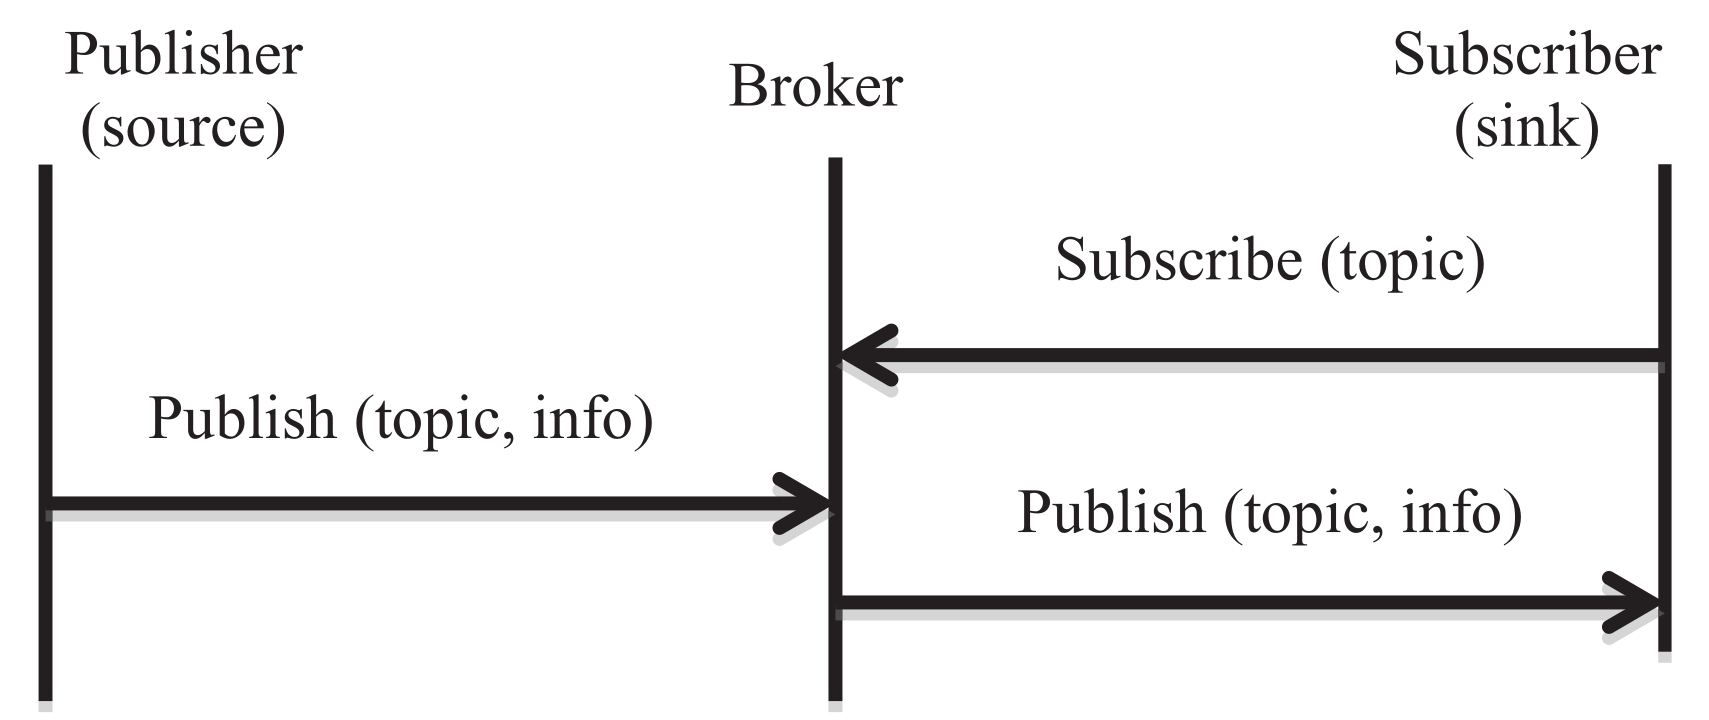
\includegraphics[width=.70\linewidth]{img/mqtt-sequence.png}
		\caption{Fonte:\cite{al-fuqaha:et-al:2015}}
	\end{figure}
\end{frame}

\begin{frame}
	\frametitle{Tópicos \mqtt}
	Ao publicar um dado no \broker \mqtt, o produtor de dados especifica um tópico onde este dado será publicado.
	O tópico pode possuir um ou mais níveis de hierarquia, com cada nível sendo separado por uma barra, como:
	\begin{itemize}
		\item \texttt{thailand/humidity};
		\item \texttt{thailand/bangkok/traffic}.
	\end{itemize}
\end{frame}

\begin{frame}
	\frametitle{Tópicos \mqtt}
	Também existe a conveniência da utilização de caracteres coringas para a assinatura de tópicos.
	Os caracteres disponíveis são:
	\begin{itemize}
		\item ``\texttt{+}'': Substitui um nível na hierarquia;
		\item ``\texttt{\#}'': Substitui todos os níveis subsequentes na hierarquia;
	\end{itemize}
	
	Como exemplo: o tópico ``\texttt{thailand/+/traffic}'' pode ser utilizado para receber os dados de tráfego de qualquer cidade da Tailândia~\cite{hunkeler:truong:stanford-clark:2008}.
\end{frame}

\begin{frame}
	\frametitle{Tópicos \mqtt}
	Dado o seguinte tópico \texttt{a/b/c/d}, as seguintes assinaturas irão receber os dados publicados nele \cite{light:mosquitto}:
	\begin{itemize}
		\item \texttt{a/b/c/d};
		\item \texttt{\#};
		\item \texttt{a/\#};
		\item \texttt{a/b/\#};
		\item \texttt{a/b/c/\#};
		\item \texttt{+/b/c/\#}.
	\end{itemize}

	
\end{frame}

\begin{frame}
	\frametitle{\mhubcddl}
	\begin{itemize}
		\item composição de um \gateway (\mhub) e um \middleware de \iomt (\cddl);
			
		\item o \mhub transforma o dispositivo \android em um \gateway \iot móvel responsável pela descoberta e aquisição de dados diretamente dos \smartobjs
			
		\item o \cddl funciona como \middleware provendo serviços locais e remotos de descoberta de provedores de serviços, processamento de eventos complexos, publicação e assinatura de dados e eventos com qualidade de serviço.
	\end{itemize}
\end{frame}

\begin{frame}
	\frametitle{Arquitetura do \mhubcddl}
	\begin{figure}
		\centering
		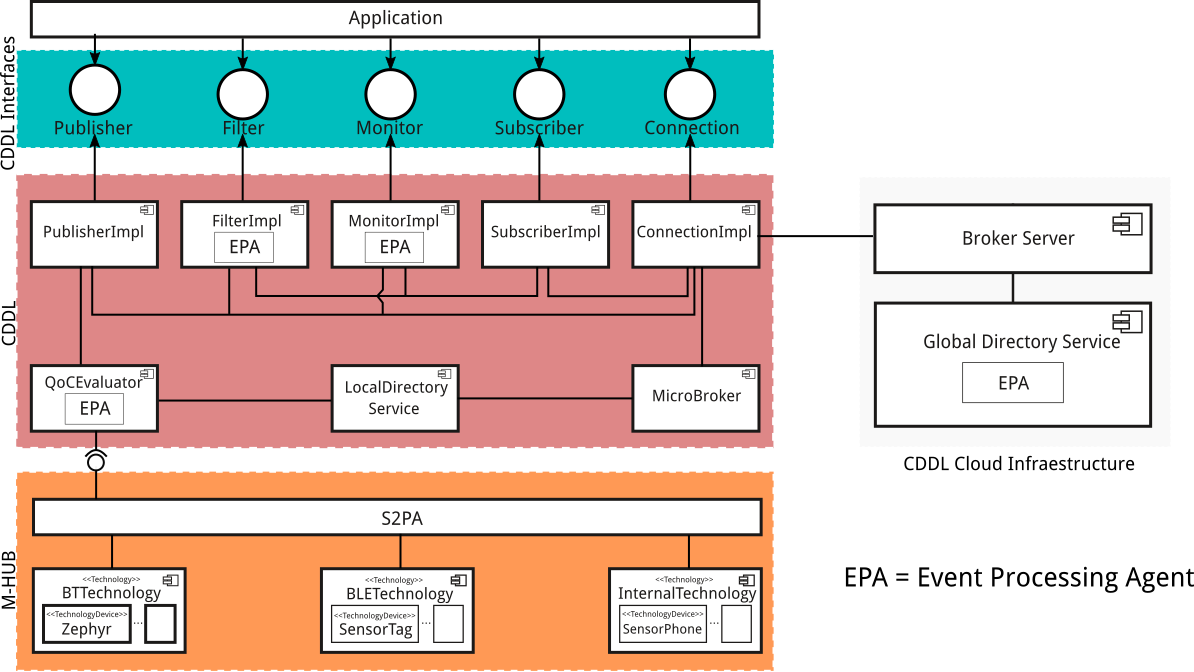
\includegraphics[width=.72\linewidth]{img/mhub-cddl-architecture.png}
		\caption{Fonte: \cite{gomes:et-al:2017}}
	\end{figure}
\end{frame}

\begin{frame}
	\frametitle{\mhub}
	Pode ser definido como um serviço de \middleware de \iomt executado em um dispositivo móvel pessoal, responsável por descobrir e oportunisticamente conectar à \smartobjs acessíveis apenas através de tecnologias WPAN de curto alcance \cite{talavera:et-al:2015}.

	\bigskip
	
	O \smartphone executando o \mhub, funciona como \gateway para \smartobjs, fornecendo acesso à Internet para dispositivos que não podem se conectar.
\end{frame}

\begin{frame}
	\frametitle{\stwopa}
	\begin{itemize}
		\item protocolo que fornece uma \api comum para realizar a comunicação com diferentes tecnologias WPAN;
			
		\item implementado como um módulo na arquitetura do \middleware, define um conjunto de métodos e interfaces que os módulos responsáveis por determinada tecnologia de comunicação devem implementar;
			
		\item fornece uma \api unificada para todas as camadas superiores da arquitetura que precisam se comunicar com tais tecnologias.
			
	\end{itemize}
	
\end{frame}

\begin{frame}
	\frametitle{Interfaces definidas pelo \stwopa}
	\begin{figure}[htb]
		\centering
		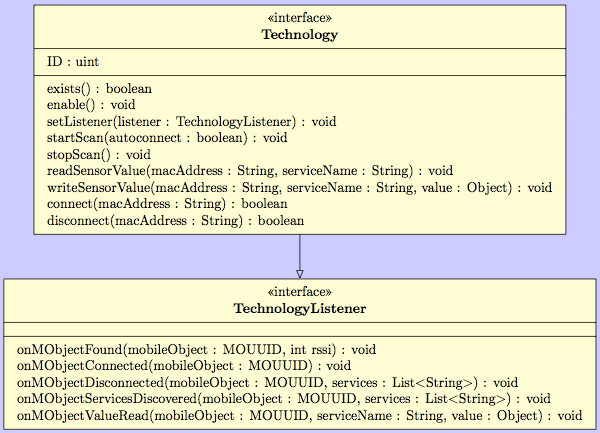
\includegraphics[width=0.55\linewidth]{img/technology-interface.png}
		\caption{Fonte: \cite{talavera:et-al:2015}}
	\end{figure}
\end{frame}

\begin{frame}
	\frametitle{\sensordata}
	Ao receber um evento de descoberta, conexão, desconexão ou leitura de dados, o \stwopa encapsula esta informação em um objeto do tipo \sensordata, possuindo os seguintes atributos:
	\begin{itemize}
		\item \texttt{mouuid}

		\item \texttt{signal}

		\item \texttt{sensorName}

		\item \texttt{sensorValue}
			
		\item \texttt{action}
		\begin{itemize}

			\item \texttt{FOUND}

			\item \texttt{CONNECTED}

			\item \texttt{READ}

			\item \texttt{DISCONNECTED}

		\end{itemize}
	\end{itemize}
\end{frame}

\begin{frame}
	\frametitle{\cddl}
	\Middleware \iomt que permite que as aplicações clientes assumam papel de produtoras ou consumidoras de dados de contexto.
	
	\bigskip
	A interação entre produtores e consumidores se dá através do modelo \pubsub com a utilização de \brokers, implementando uma comunicação distribuída com o \mqtt.
	\bigskip
	
	Fornece também um \ubroker que executa internamente no dispositivo móvel.
\end{frame}

\begin{frame}
	\frametitle{A classe \msg}
	Ao receber do \mhub um instância de \sensordata, está é convertida para uma instância de \msg, uma classe interna do \cddl.
	Todos os dados publicados pelo \cddl são intâncias desta classe. Dentre seus atributos, destaca-se:
	\begin{itemize}
		\item \texttt{serviceName}

		\item \texttt{serviceValue}

		\item \texttt{accuracy}

		\item \texttt{sourceLocationLatitude}

		\item \texttt{sourceLocationLongitude}

		\item \texttt{signal}
	\end{itemize}
	Toda instância de \msg gerada é automaticamente publicada em um \broker.
\end{frame}

\begin{frame}
	\frametitle{Visão geral do \mhubcddl}
	\begin{figure}
		\centering
		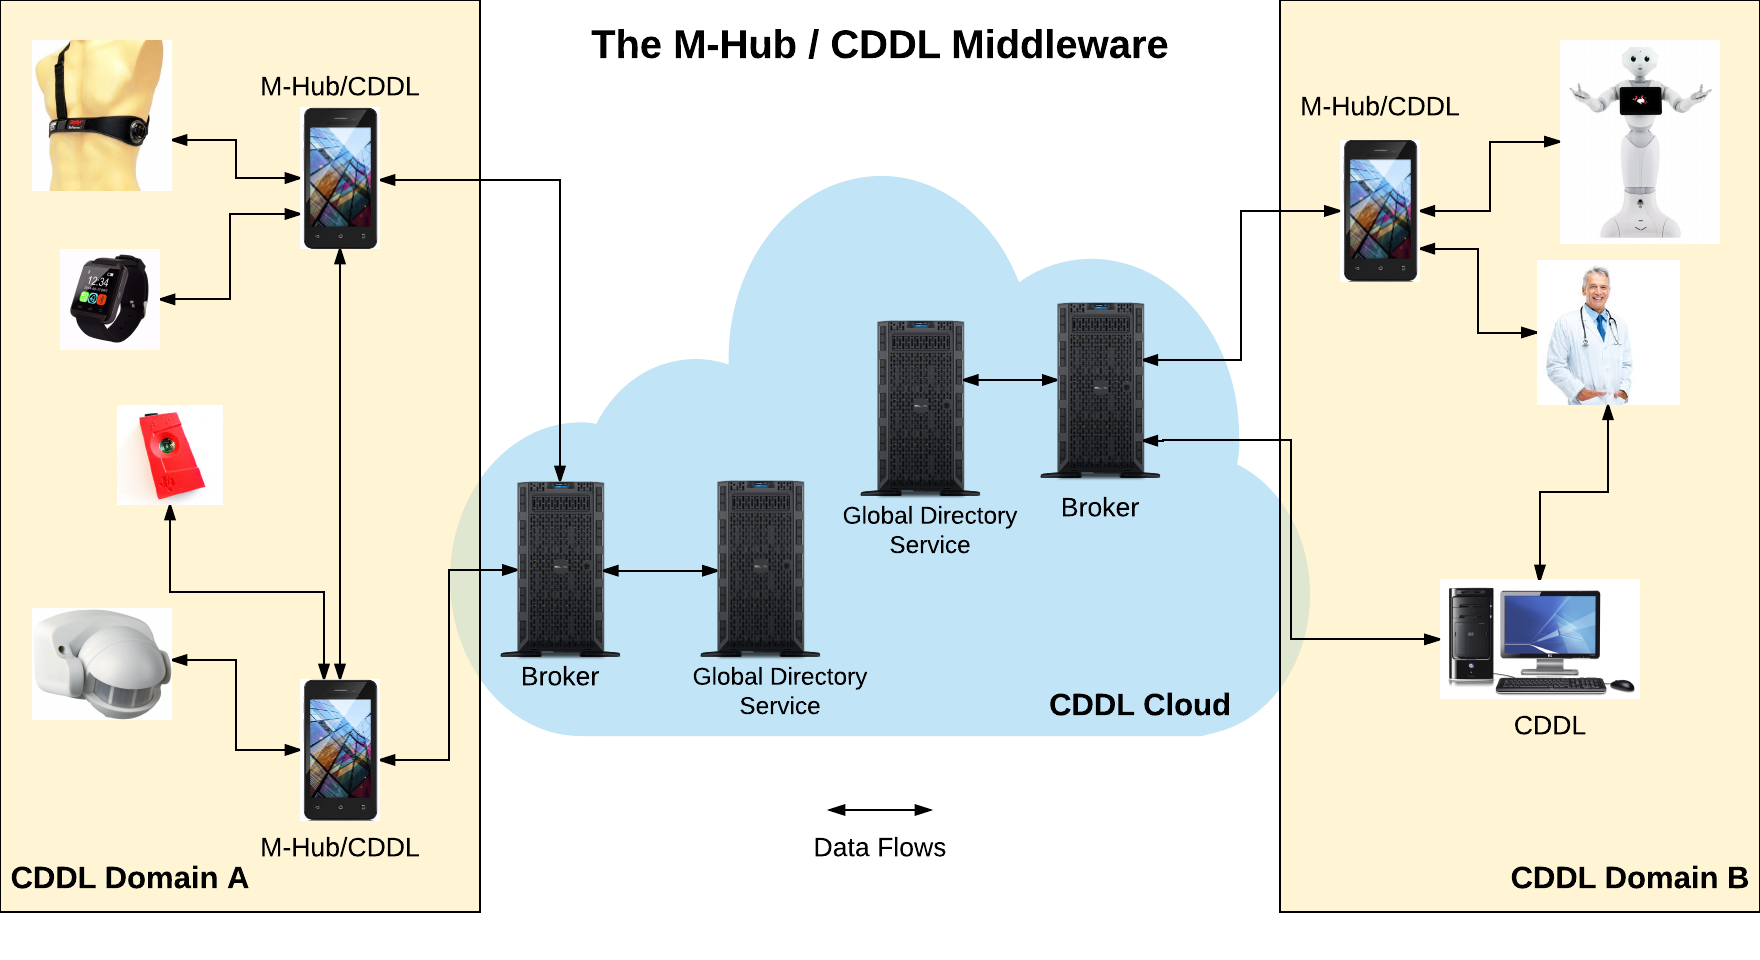
\includegraphics[width=0.70\linewidth]{img/general-vision-cddl.png}
		\caption{Fonte: \cite{gomes:2017}}
	\end{figure}
\end{frame}


\section{Solução proposta}


\begin{frame}
	\frametitle{Contexto}
	Dado o fato que o \cddl somente envia à camada de aplicação dados referentes à leitura de dados, as seguintes implicações ocorrem no desenvolvimento de aplicações:
	\begin{itemize}
		\item incapacidade de gerenciar efetivamente recursos computacionais;

		\item limitações no desenvolvimento de aplicações que não interagem com \smartobjs por meio de conexões.
	\end{itemize}
\end{frame}

\begin{frame}
	\frametitle{Requisitos}
	\begin{itemize}
		\item notificação de eventos de descoberta, conexão e desconexão de \smartobjs para a camada de aplicação do \software;

		\item separação dos fluxos de eventos, provendo uma \api que permita a aplicação registrar interesse em cada tipo de evento individualmente;

		\item permitir que estes eventos possam estar acessíveis tanto para a aplicação que os gera, quanto para aplicações remotas que registrem interesse em interações de outros \smartphones com \smartobjs;

		\item fornecer uma \api assíncrona para o recebimento de cada notificação dos eventos desejados.
	\end{itemize}
\end{frame}

\begin{frame}
	\frametitle{Propagação dos eventos do \stwopa ao \cddl}
	Foi realizada uma modificação no \stwopa do \mhub para que este publique os objetos \sensordata que representem eventos de descoberta, conexão e desconexão com \smartobjs.

	\bigskip

	A comunicação é realizada através de \eventbus.
\end{frame}

\begin{frame}
	\frametitle{Separação do fluxos de eventos}
	Como todos os dados publicados pelo \cddl são do tipo \msg, decidiu-se utilizar uma estratégia diferente da tomada pelo \stwopa para representar diferentes tipos de eventos.

	\bigskip

	Adotou-se uma estratégia baseada em orientação a objetos, onde as seguintes classes que herdam \msg foram criadas:
	\begin{itemize}
		\item \objfoundmsg;
		\item \objconnectedmsg;
		\item \objdisconnectedmsg;
		\item \sensordatamsg.
	\end{itemize}
\end{frame}

\begin{frame}
	\frametitle{Definição da estrutura de tópicos}
	Cada mensagem deve ser publicada em um tópico específico, de acordo com o tipo de evento que esta representa.

	\bigskip

	A estrutura de tópicos proposta para publicação de eventos de descoberta, conexão e desconexão segue o seguinte padrão:
	\[
		\underbrace{\bm{\mathsf{domain}}\vphantom{p}}_{\text{\textsf{identificador do \cddl}}}
		\bm{/}
		\underbrace{\bm{\mathsf{clientId}}\vphantom{p}}_{\text{\textsf{identificador do cliente}}}
		\bm{/}
		\underbrace{\bm{\mathsf{eventTopic}}}_{\text{\textsf{identificador do tipo de evento}}}
	\]
\end{frame}

\begin{frame}
	\frametitle{Definição da estrutura de tópicos}
	Caso seja necessário receber notificações de eventos provenientes de outras aplicações, pode-se fazer uso dos caracteres coringa do \mqtt, como:
	\texttt{domain/+/eventTopic}.
\end{frame}

\begin{frame}
	\frametitle{Diagrama de sequência}
	\begin{figure}
		\centering
		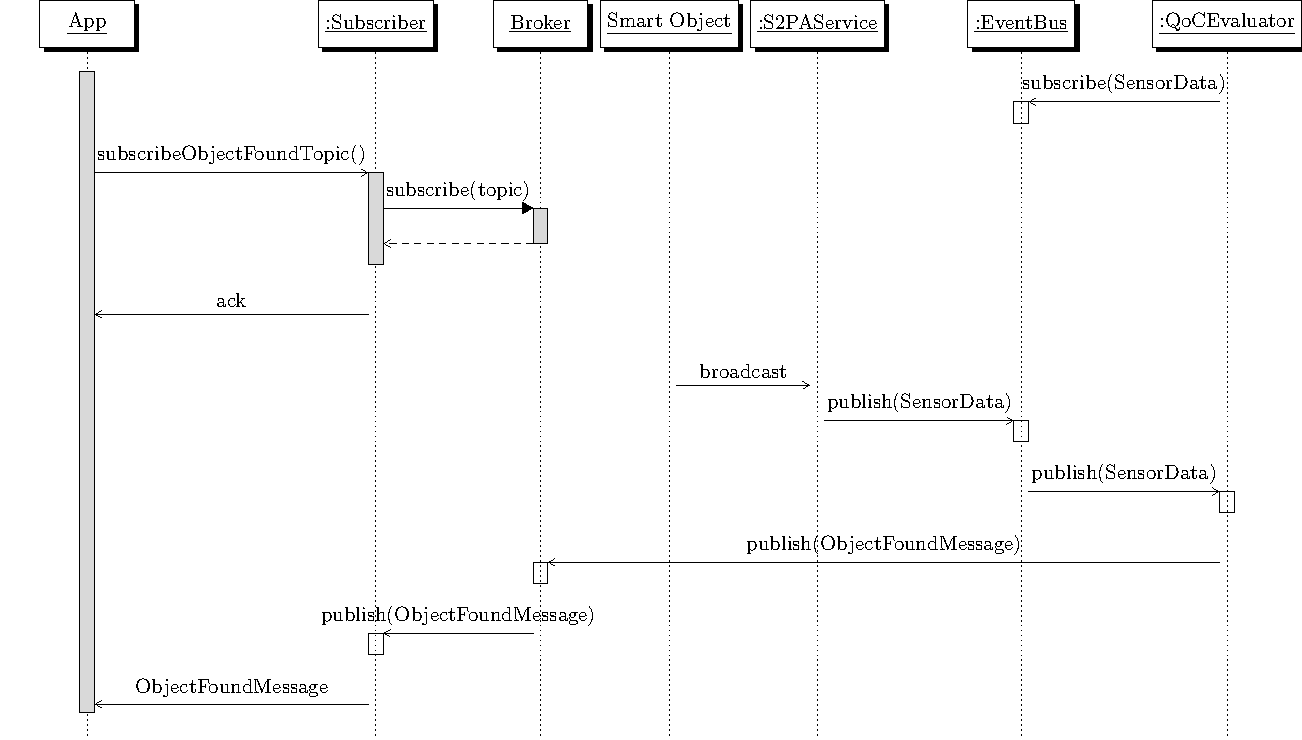
\includegraphics[width=.85\linewidth]{img/solution-sequence.pdf}
	\end{figure}
\end{frame}

\begin{frame}
	\frametitle{Extensão da \api}
	Foram adicionados novos métodos à interface \texttt{Subscriber} que permitem que a aplicação registre interesse nos novos eventos, são elas:
	\begin{itemize}
		\item \texttt{subscribeObjectFoundTopic()}:

		\item \texttt{subscribeObjectConnectedTopic()}:

		\item \texttt{subscribeObjectDisconnectedTopic()}:
	\end{itemize}
\end{frame}


\section{Avaliação quantitativa}


\begin{frame}
	\frametitle{Objetivos}
	As avaliações têm como objetivo determinar a performance e o percentual de perdas de notificações de eventos de interações com \smartobjs.

	\bigskip

	Serão feitos experimentos baseados em cenários de uso.
\end{frame}

\begin{frame}
	\frametitle{Experimento 1}
	Se propõe a analisar a performance e o percentual de perdas de notificações de eventos de descobertas de \smartobjs.

	\bigskip
	
	Métricas a serem utilizadas:
	\begin{equation}
		\label{equ:performance-discovery}
		\Delta t_{descoberta} = t_{descoberta,app} - t_{descoberta,\stwopa}
	\end{equation}
	
	\begin{equation}
		\label{equ:acuracy}
		P_{perda} = \frac{EventosGerados - EventosNotificados}{EventosGerados} \cdot 100
	\end{equation}
\end{frame}

\begin{frame}
	\frametitle{Processo de medição}
	\begin{figure}
		\centering
		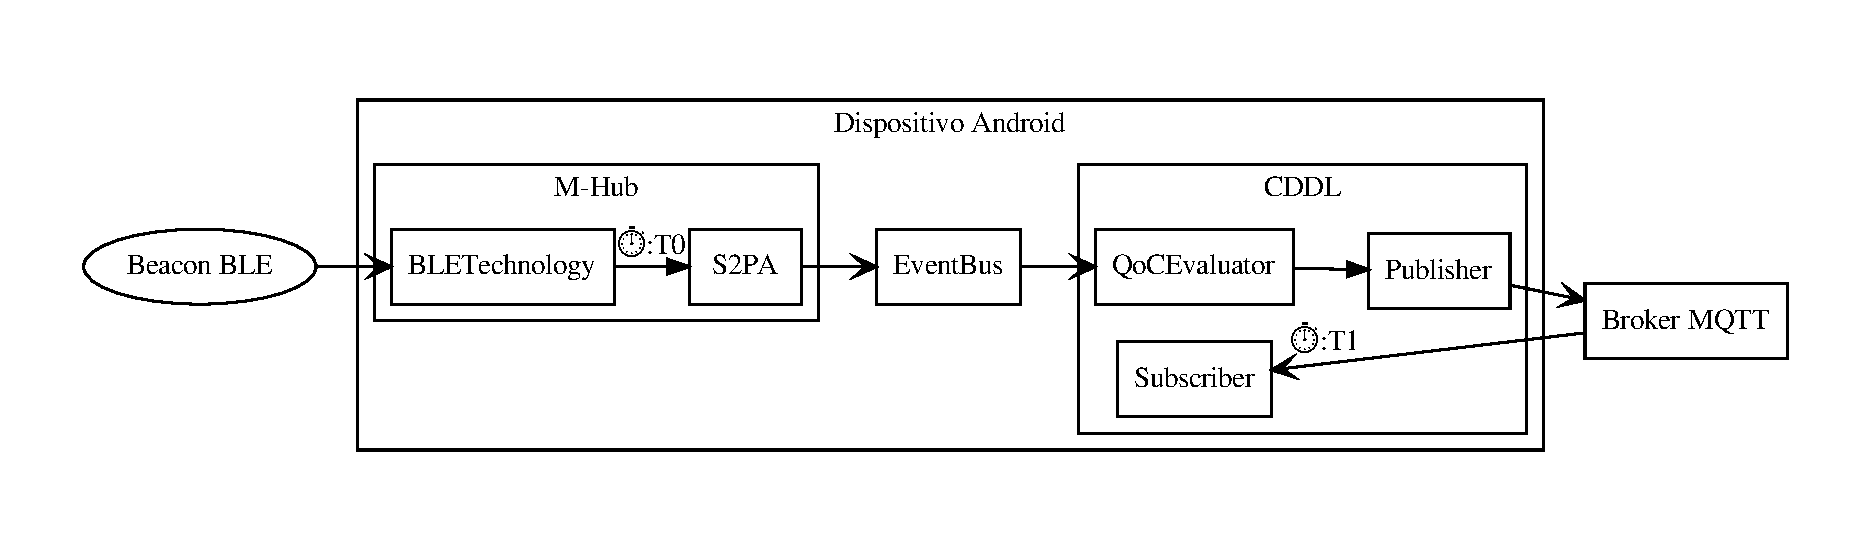
\includegraphics[width=.85\linewidth]{img/performance-annotation.pdf}
	\end{figure}
\end{frame}

\begin{frame}
	\frametitle{Cenário}
	Consiste em uma casa onde cada cômodo possui um \beacon \ble e o morador é instruído a conduzir suas atividades do dia a dia.

	\bigskip
	
	O morador possui um \smartphone executando uma aplicação \mhubcddl, e cada vez que entra em um cômodo o \beacon será descoberto e um evento será gerado no \stwopa.

	\bigskip
	
	Cada \beacon está configurado para emitir 10 anúncios por segundo.
\end{frame}

\begin{frame}
	\frametitle{Simulação da locomoção na residência}
	Os dados utilizados para a simulação de locomoção de um indivíduo em uma residencia foram obtidos através de um \dataset disponibilizado em \cite{byrne:et-al:2018}.

	\bigskip

	Neste trabalho a locomoção de moradores em suas residências foi monitorada com o auxílio de câmeras e marcadores.
\end{frame}

\begin{frame}
	\frametitle{Frequência de entrada por cômodo}
	\begin{figure}
		\centering
		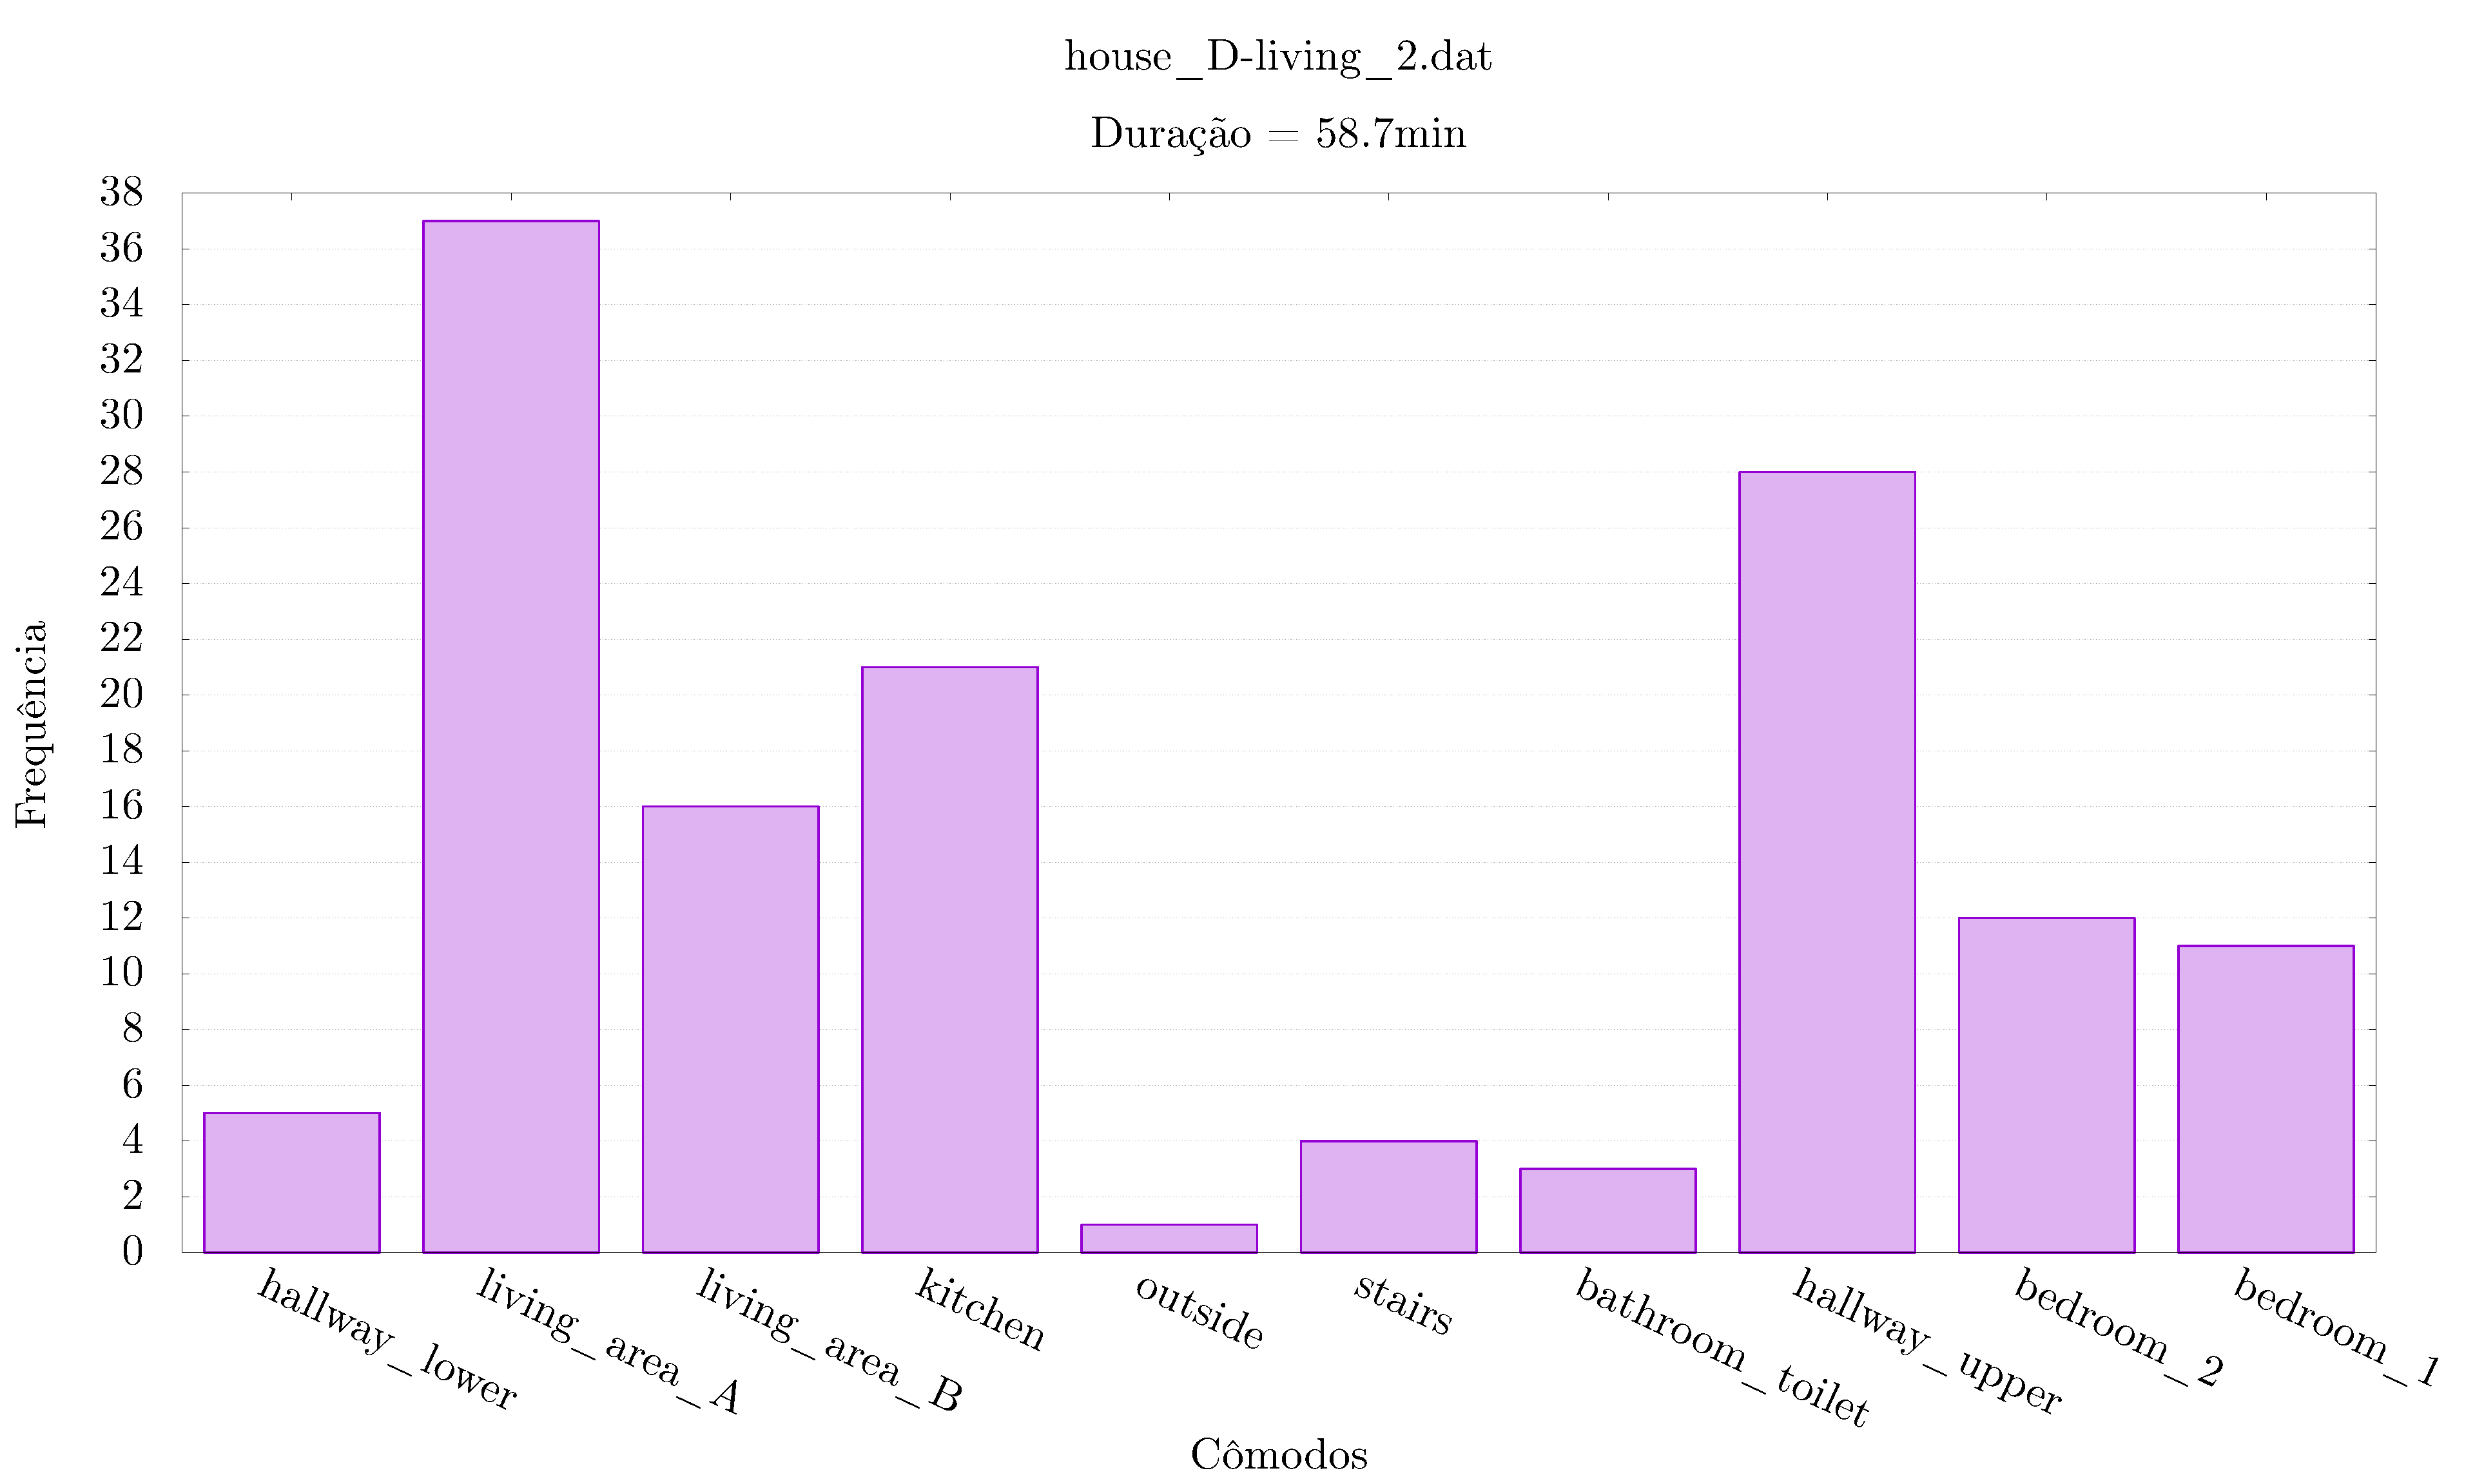
\includegraphics[width=.80\linewidth]{img/dataset-histogram.pdf}
	\end{figure}
\end{frame}

\begin{frame}
	\frametitle{Simulação do \beacons}
	Utilizando o \dataset já descrito, a cada momento em que o participante entra em determinado cômodo, calcula-se a quantidade de anúncios o \beacon daquele cômodo transmitirá durante o tempo de permanência no local, o cálculo é apresentado a seguir.
	
	\begin{equation}
		anuncios = \frac{tempoPermanencia}{0.1} 
	\end{equation}
\end{frame}

\begin{frame}
	\frametitle{Quantidade de eventos gerados}
	\begin{table}
		\centering
		\begin{tabular}{lc}
			\toprule
						       & $EventosGerados$ \\
			\midrule 
			\textbf{Eventos de descoberta} & 34814            \\
			\textbf{Eventos de conexão}    & 0                \\
			\textbf{Eventos de desconexão} & 0                \\
			\bottomrule
		\end{tabular}
	\end{table}
\end{frame}

\begin{frame}
	\frametitle{Resultados}
	\newcommand{\nullval}{\textbf{---}}

	\begin{table}[htb]
		\begin{center}
			\begin{tabular}{lccc}
				\toprule
							       & $EventosGerados$ & $EventosNotificados$ & $P_{perdas}$ (\%) \\
				\midrule
				\textbf{Eventos de descoberta} & 34814            & 34814                & 0		     \\
				\textbf{Eventos de conexão}    & 0                & 0                    & \nullval	     \\
				\textbf{Eventos de desconexão} & 0                & 0                    & \nullval          \\
				\bottomrule
			\end{tabular}
		\end{center}
	\end{table}

	\bigskip

	\begin{table}[htb]
		\centering
		\begin{adjustbox}{max width=\textwidth}
			\begin{tabular}{lccccc}
				\toprule
									   & Média & Desvio padrão & Mínimo & Máximo & Intervalo de 95\% de confiança \\
				\midrule
				$\bm{\Delta t_{descoberta}}$ \textbf{(ms)} & 20.1  & 3.7           & 7.0 & 78.9 & 20.1 $\pm$ 0.03 	              \\
				\bottomrule
			\end{tabular}
		\end{adjustbox}
	\end{table}

\end{frame}

\begin{frame}
	\frametitle{Análise dos resultados}
	Mesmo com os \beacons configurados para emitir um \broadcast a cada 0.1 segundo, a solução conseguiu notificar a aplicação com tempos na casa de milissegundos. Este tempo pode ser considerado desprezível para aplicações reais.

	\bigskip

	Do ponto de vista de percentual de perdas, a pesar do grande número de eventos, não houve nenhuma perda de notificação.
\end{frame}

\begin{frame}
	\frametitle{Experimento 2}
	Se propõe a analisar a performance e o percentual de perdas, mas levando em consideração eventos de conexão que não foram considerados no experimento anterior.

	\bigskip

	Métricas a serem utilizadas:
	
	\begin{align}
		\label{equ:performance-ready}
		\Delta t_{conectado} &= t_{conexao,app} - t_{descoberta,\stwopa}
	\end{align}
	
	\begin{equation}
		P_{perda} = \frac{EventosGerados - EventosNotificados}{EventosGerados} \cdot 100
	\end{equation}
\end{frame}

\begin{frame}
	\frametitle{Cenário}
	Consiste em uma casa equipada com um sistema multimídia na sala de estar que possibilita que \smartphones se conectem a ele através de \bluetooth.

	\bigskip

	O sistema multimídia pode ter ciência de qual usuário está presente através dos \smartphones conectados no momento, pois ele armazena a relação dos moradores da residência com seus respectivos \smartphones.

	\bigskip

	Uma aplicação \android foi desenvolvida com o \middleware \mhubcddl que permanece ativamente procurando e se conectando ao sistema multimídia no ambiente.
\end{frame}

\begin{frame}
	\frametitle{Simulação do sistema multimídia}
	Foi utilizado o mesmo \dataset do experimento anterior para simular uma pessoa se locomovendo em uma casa.

	\bigskip

	O sistema multimídia foi posicionado no cômodo \texttt{living\_area\_A}.

	\bigskip

	Ao entrar neste cômodo, ocorre um evento de descoberta seguido de um evento de conexão. Ao sair do cômodo um evento de desconexão é gerado.
\end{frame}

\begin{frame}
	\frametitle{Quantidade de evento gerados}
	\begin{table}[htb]
		\begin{center}
			\begin{tabular}{lc}
				\toprule
							       & $EventosGerados$ \\
				\midrule 
				\textbf{Eventos de descoberta} & 37               \\
				\textbf{Eventos de conexão}    & 37               \\
				\textbf{Eventos de desconexão} & 37               \\
				\bottomrule
			\end{tabular}
		\end{center}
	\end{table}
\end{frame}

\begin{frame}
	\frametitle{Resultados}
	\begin{table}[ht]
		\centering
		\begin{tabular}{lccc}
			\toprule
						       & $EventosGerados$ & $EventosNotificados$ & $P_{perdas}$ (\%) \\
			\midrule
			\textbf{Eventos de descoberta} & 37               & 37                   & 0		     \\
			\textbf{Eventos de conexão}    & 37	          & 37                   & 0		     \\
			\textbf{Eventos de desconexão} & 37	          & 37                   & 0	             \\
			\bottomrule
		\end{tabular}
	\end{table}

	\bigskip

	\begin{table}[ht]
		\centering
		\begin{adjustbox}{max width=\textwidth}
			\begin{tabular}{lccccc}
				\toprule
							  & Média & Desvio padrão & Mínimo & Máximo & Intervalo de 95\% de confiança \\
				\midrule
				$\bm{\Delta t_{conectado}}$ \textbf{(ms)} & 501.4 & 60.8         &425.1        & 654.5       &	501.4 $\pm$ 19.6	                  \\
				\bottomrule
			\end{tabular}
		\end{adjustbox}
	\end{table}

\end{frame}

\begin{frame}
	\frametitle{Análise dos resultados}
	
	Não foi possível observar perda de notificações neste experimento.

	\bigskip
	
	O tempo entre a descoberta de um \smartobj no ambiente e sua conexão se manteve em torno de 500 milissegundos.

	\bigskip

	Isto implica que uma aplicação que necessite de dados oferecidos por sensores no ambiente, começaria a receber estes dados em média 0.5 segundo após o primeiro encontro com este dispositivo.

	\bigskip

\end{frame}

\begin{frame}
	\frametitle{Análise dos resultados}
	Em um cenário onde uma aplicação necessita de dados de um sensor em um poste público, e assumindo que o raio do \smartobj é de 5 metros:

	\[
		\frac{10\si{\meter}}{0.5\si{\second}} = 20\si{m/s} = 72\si{km/h}
	\]

\end{frame}


\section{Trabalhos futuros}


\begin{frame}
	\frametitle{Trabalhos futuros}
	Como trabalhos futuros, prevê-se:
	\begin{itemize}
		\item novas avaliações que possam responder sobre a performance da solução ao utilizar um \broker em rede;

		\item avaliar a capacidade de escalabilidade da solução.
	\end{itemize}
\end{frame}


\section{Referências}

\begin{frame}[allowframebreaks]
	\frametitle{Referências}
	\bibliographystyle{apalike}
	\bibliography{bib/biblio}
\end{frame}

\end{document}
